
%...........................................................
%
% Comparison between 1D Ereco and 2D Ereco Vs Theta templates
%
%...........................................................

\section{Impact of 1D $E_{reco}$ and 2D $E_{reco}$ vs $\theta$ templates}
\label{app:comp_1d_ereco_2d_ereco_vs_theta}

It has been checked that using 1- or 2- dimensional 
templates does not make any difference in the 
drawing of the error envelopes and the effect of the systematic
uncertainties on the total number of events.
The uncertainty on the total number of events due to the flux, cross section, Super-K-FSI-SI systematic parameters, 
i.e. the systematic uncertainties which have a dependence on $\theta$,
are shown in \cref{tab:syst_diff_2d_1d_templates}.
The fractional errors of $E_{reco}$ and $E_{reco}$ vs $\Theta$ templates are in very good agreement.
This table also shows that there is no problem with fitting $E_{reco}$ and $\theta$ if the correlations between the two variables 
are correctly taken into account. 
Indeed when the lepton angle variable is averaged out the same uncertainty as in the $E_{reco}$ only template is obtained.

\begin{table}
\centering
 \begin{tabular}{| c | c | c |}
 \hline
 Super-K sample                                               	& 2D $E_{reco}$ vs $\theta$	  	& 1D $E_{reco}$ only   \\
\hline
antineutrino mode $e$-like                                	& 4.64\%						& 4.59\%   \\
neutrino mode $e$-like                                       & 4.19\%						& 4.11\%   \\
antineutrino mode $\mu$-like                             & 3.29\%     					& 3.34\%     \\
neutrino mode $\mu$-like                            	& 2.89\%		    				& 2.94\%     \\
\hline
\end{tabular}
\caption{
Effect of 1$\sigma$ variations on the total number of events given by flux, cross section and Super-K+FSI+SI+PN systematic uncertainties
obtained by performing 10k toys MC.
The RMS / Mean of the distribution is assumed to be the $1\sigma$ uncertainty.
The systematic parameter values measured with the ND280 data 
shown in 
\cref{tab:banff_uncertainties_flux_fhc},
~\ref{tab:banff_uncertainties_flux_rhc}
~\ref{tab:banff_uncertainties_xsec}
and
~\ref{tab:banff_uncertainties_skdetfsi}
and the oscillation parameters of the Asimov data set A shown in \cref{tab:osc_params_joint_asimov}
are used.
}
\label{tab:syst_diff_2d_1d_templates}
\end{table}


In \cref{fig:joint_data_fit_dcp_comp_oa_groups} the comparison of the results between the oscillation analysis 
groups (VALOR, Mach3 and p-$\theta$) is shown.
The VALOR analysis agrees with the p-$\theta$ result if 2D $e$-like templates are used.
If 1D $E_{reco}$ templates are used, the significance to $\delta_{CP}$ becomes weaker and for 
$\delta_{CP} = +\pi/2$ the $\delta \chi^2$ is smaller by $\sim 1$ and agrees perfectly with the Mach3 analysis.
This is due to the powerful of the reconstructed lepton angle information which allows to 
better distinguish the $\nu_{\mu} \rightarrow \nu_e$ and $\bar{\nu}_{\mu} \rightarrow \bar{\nu}_e$ components,
as shown in appendix~\ref{app:templates_elike}.

\begin{figure*}[htb]
\center
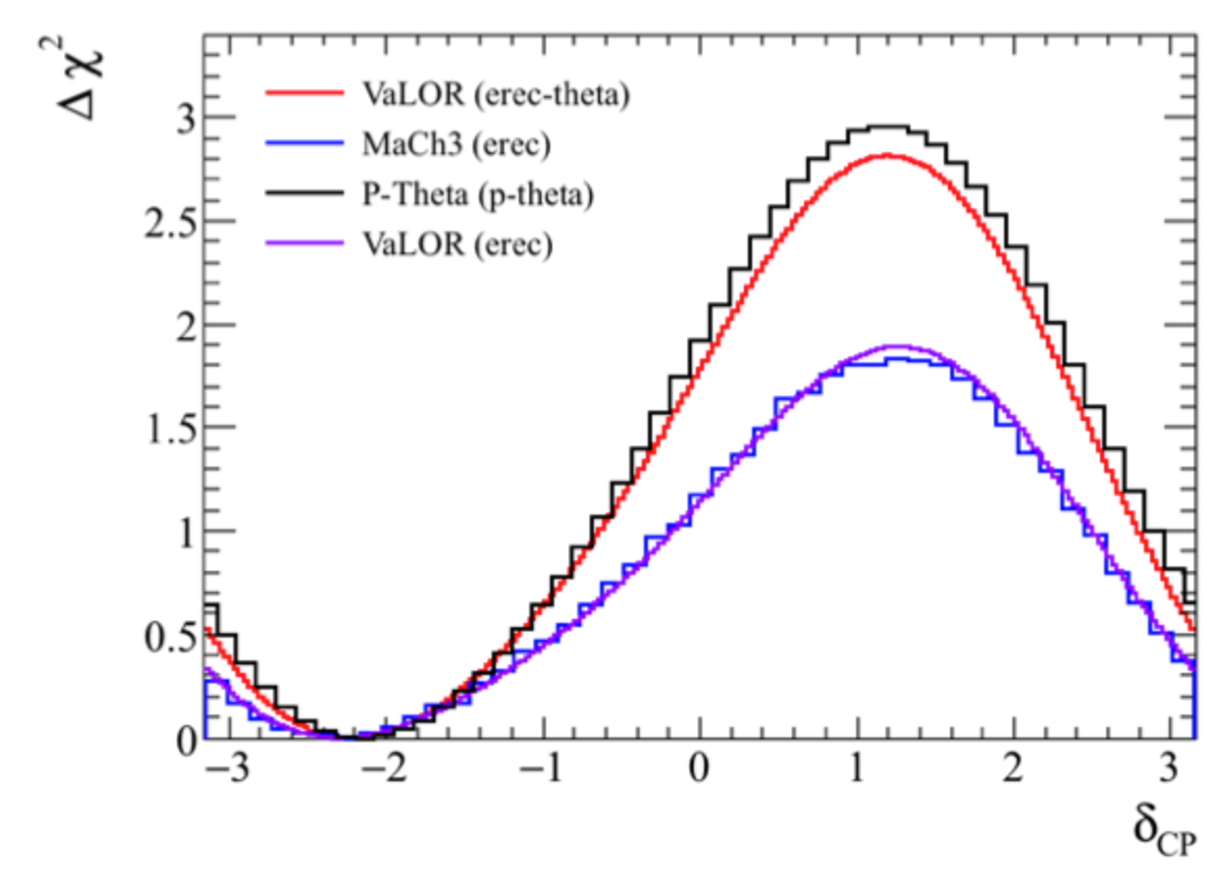
\includegraphics[width=0.49\textwidth]{joint_plots/data_contours/Ereco_ErecoVsTheta.pdf}
\caption{$\delta_{CP}$ with reactor constraint}
\caption{
Measured $\Delta \chi^2$ distributions
with the full Run 1-6 data set with T2K only data.
Normal hierarchy is shown. 
The current analysis result is shown for 1D $E_{reco}$ only $e$-like template (purple)
as well as for 2D $E_{reco}$ vs $\theta$ $e$-like templates.
The result of the Mach3 \cite{Mach3JointFitRun16} analysis is shown by the blue line, 
while the result of the p-$\theta$ \cite{ptheta} analysis is shown by the black line.
}
\label{fig:joint_data_fit_dcp_comp_oa_groups}
\end{figure*}




\clearpage


